 \documentclass{openetcs_article}
% Use the option "nocc" if the document is not licensed under Creative Commons
%\documentclass[nocc]{template/openetcs_article}
\usepackage{todonotes}
\usepackage{lipsum,url}
\usepackage{pdfpages}
\usepackage{bibtopic} % Multibib
\usepackage{booktabs}
\usepackage[hidelinks]{hyperref}
\usepackage[section, % add the glossary to the table of content 
            description,% acronyms have a user-supplied description,
            style=superheaderborder, % table style
            nonumberlist,      % no page number
]{glossaries}

%===========================
% Graphicpath
%===========================
\graphicspath{{./template/}{.}{./images/}}

%===========================
% Abbreviation file
%===========================
\renewcommand*{\glossaryname}{List of Terms}
\makeglossaries
\loadglsentries{glossary} 
%===========================

\begin{document}
\frontmatter
\project{openETCS}

%Please do not change anything above this line
%============================
% The document metadata is defined below

%assign a report number here
\reportnum{OETCS/WP7/O7.3.1}

%define your workpackage here
\wp{Work-Package 3: ``Tool chain''}

%set a title here
\title{Tool chain Development Plan}

%set a subtitle here
\subtitle{Description of the tool chain development process}

%set the date of the report here
\date{September 2013}

%define a list of authors and their affiliation here

\author{Cecile Braunstein \and Jan Peleska}

\affiliation{University Bremen}



% define the coverart
\coverart[width=350pt]{openETCS_EUPL}

%define the type of report
\reporttype{Software development Plan}


\begin{abstract}
%define an abstract here
  This document defines the development process of the openETCS tool
  chain. 

\end{abstract}

%=============================
%Do not change the next three lines
\maketitle
\tableofcontents
\listoffiguresandtables

\newpage
%=============================

% The actual document starts below this line
%=============================
%Start here
%=============================
% Document Managment
%=============================
\section*{Document Information}
\begin{tabular}{|p{4.4cm}|p{8.7cm}|}
\hline
\multicolumn{2}{|c|}{Document information} \\
\hline
Work Package &  WP7  \\
Deliverable ID or doc. ref. & O7.3.1\\
\hline
Document title & Tool chain development Plan \\
Document version & 00.02 \\
Document authors (org.)  & Cécile Braunstein  (Uni.Bremen)  \\
& Jan Peleska (Uni. Bremen)\\
\hline
\end{tabular}

\begin{tabular}{|p{4.4cm}|p{8.7cm}|}
\hline
\multicolumn{2}{|c|}{Review information} \\
\hline
Last version reviewed &  \\
\hline
Main reviewers & \\
\hline
\end{tabular}

\begin{tabular}{|p{2.2cm}|p{4cm}|p{4cm}|p{2cm}|}
\hline
\multicolumn{4}{|c|}{Approbation} \\
\hline
  &  Name & Role & Date   \\
\hline  
Written by    &  Cécile Braunstein & WP7-T7.3 Sub-Task  & \\
& Jan Peleska & Leaders&\\
\hline
Approved by & &  & \\
\hline
\end{tabular}

\begin{tabular}{|p{2.2cm}|p{2cm}|p{3cm}|p{5cm}|}
\hline
\multicolumn{4}{|c|}{Document evolution} \\
\hline
Version &  Date & Author(s) & Justification  \\
\hline  
00.01 & 29.04.2013 & C. Braunstein  &  Document creation  \\
00.01 & 26.06.2013 & C. Braunstein  &  Document correction  \\
\hline  
\end{tabular}
\newpage
%==========================================


%------ List of terms and definition ----------------
\printglossary
%==========================================
\mainmatter
%----------------------
\section{Introduction and Motivation}



%-----------------------
\section{Motivation}
%-----------------------

%-----------------------
\section{Scope of the document}
%-----------------------

%----------------------
 \section{Reference documents}
%----------------------- 
\begingroup
%\renewcommand{\section}[2]{}%
\renewcommand{\chapter}[2]{}% for other classes
  \bibliographystyle{plain}
  \bibliography{wp7_bibliography}
\endgroup
%%% Local Variables: 
%%% mode: latex
%%% TeX-master: WP7-Toolchain_architecture"
%%% End: 

%----------------------
\section{Reference documents}

\bibliographystyle{unsrt}
\begin{btSect}{intern-doc}
\subsection{Project documents}
\btPrintAll
\end{btSect}
\begin{btSect}{standards}
\subsection{Standards documents}
\btPrintAll
\end{btSect}

%----------------------
\section{OpenETCS Tool chain Definition Methods}
\label{sec:toolchaindef}
%----------------------------------------------------
\section{The OpenETCS tool chain}
%----------------------------------------------------
\subsection{Definition}
%----------------------------------------------------
The tool chain provides the tool support and the development process
to provide a formalized specification of \gls{SRS} and an executable
code of the \gls{OBU}.


The tool chain is composed by two kind of tools :
\begin{enumerate}
\item {\it Development tools}: those used along the phases of the software
  development process (Requirement engineering, modeling ...).
\item {\it Management tools}:  those used transversely during the
  complete development process (version management, requirements
  traceability ...).
\end{enumerate}
These tools are called vertical and horizontal tools in
\cite{wasserman_tool_1990}. 
Figure \ref{fig:toolchain} shows the idea of the complete tool chain
integration.

\begin{figure}[htbp]
\centering
  \includegraphics[width=.5\textwidth]{images/toolchain_archi-dev}
  \caption{The OpenETCS tool chain}
  \label{fig:toolchain}
\end{figure}

In the next chapters  we will give more details on the
data integration between the development tools by defining the inputs
and outputs artifact of each tools. This document describes the
interface between the tool chain activities.
The interoperability mechanism will be defined in a separate
document. However, the first version of the tool chain will implement a
file-based data exchange.
 
It has been decided (see \cite{D7.1}) that the tool platform hosting
the tool chain is Eclipse with the Eclipse modeling framework
(\gls{EMF}).  This implies that the tool chain will be a set of
Eclipse plug-ins. It also implies that we can rely on already
available plug-in and features for the versioning, the project
management or the build system.  The use of EMF will also assist the
software development, by providing a meta model and an \gls{API} for
manipulating EMF components.


%----------------------------------------------------
\subsection{The SysML Model}
%----------------------------------------------------
A SysML model of the tool shown figure \ref{fig:overview} . It
allows us to have a formal representation of the tool chain and
help to model precisely the different interaction between the
development tools as well as the management tools.  The SysML model
may be also seen as a guideline for integrated new tool: each new tool
should be fully described and comply to the defined interfaces.
Moreover following the idea of Slotosch \cite{slotosch_iso_2012} the
model will be the basis to the qualification analysis \cite{D7.3}.

\begin{figure}[htbp]
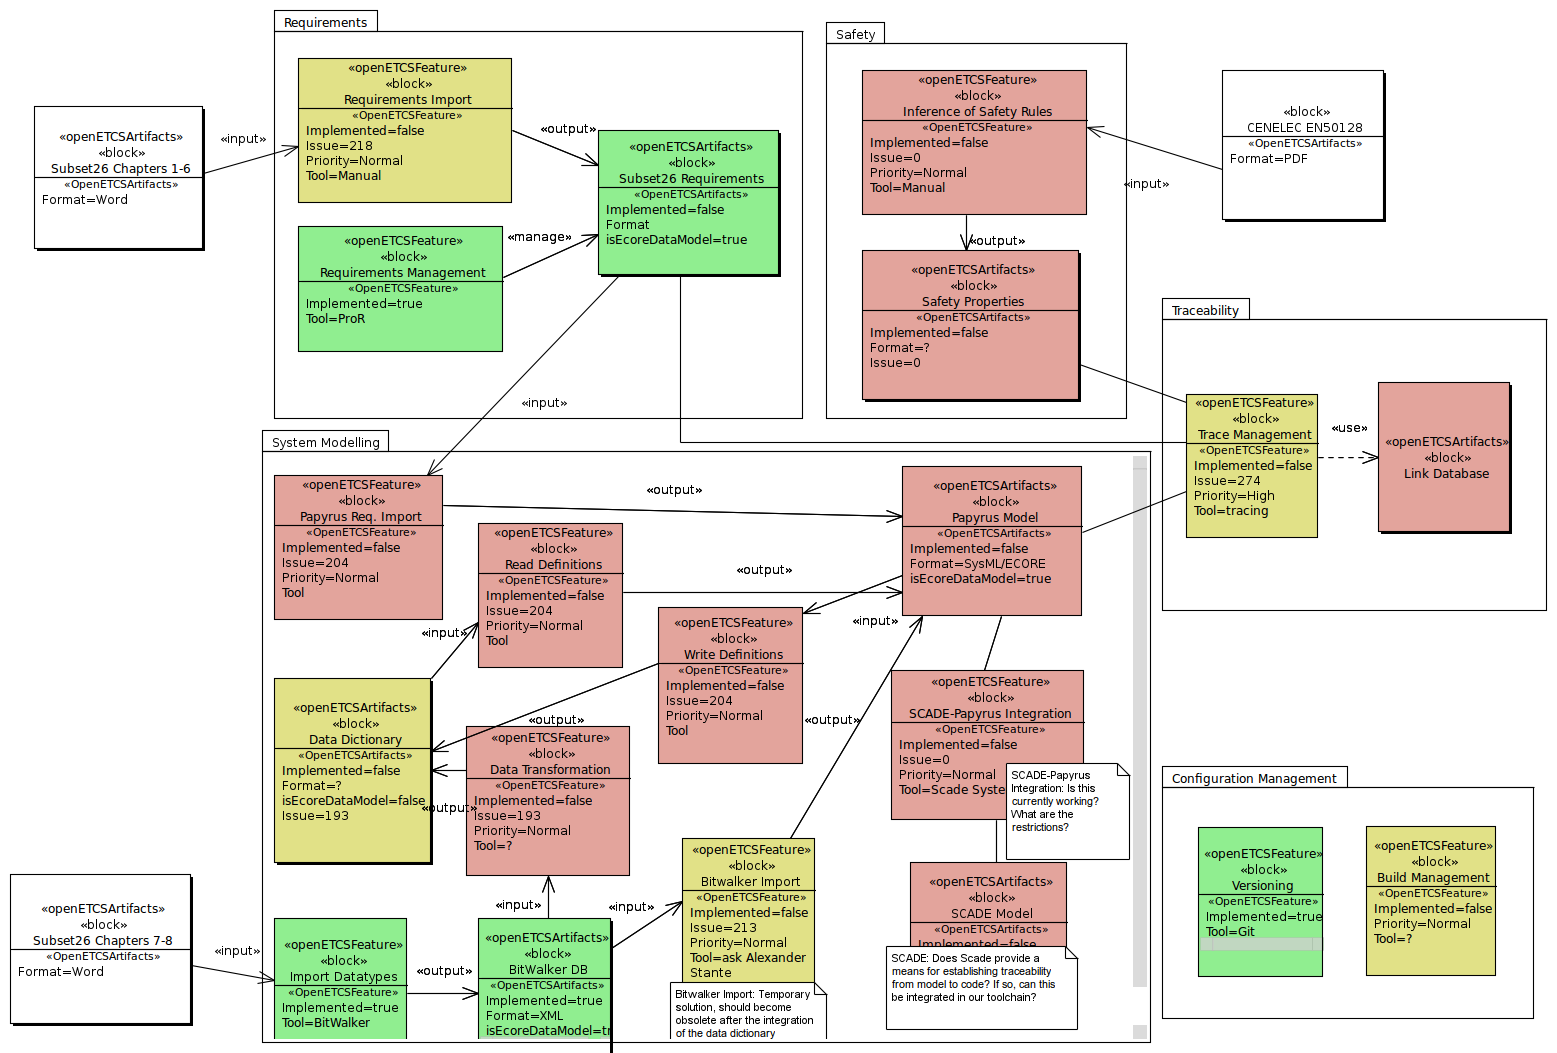
\includegraphics[width= \textwidth]{images/ToolChainmodel.png}
\caption{\label{fig:overview}OpenETCS tool chain Status Overview}
\end{figure}
\todo[inline]{Check if the overview is up-to-date and complient with
  the real implementation}

The requirements of WP2 \cite{baro_requirements_2013} as well as our
intern requirements (Appendixes \ref{app:wp2req} and \ref{app:WP7Req})
will be included in the SysML model. Each tools and their connections
should then also comply to the requirements list.


%----------------------------------------------------
\subsection{The OpenETCS lifecycle}
%----------------------------------------------------
\todo[inline]{Insert the tool chain lifecycle definition from WP1}
%----------------------------------------------------
\section{OpenETCS \gls{EVC} lifecycle}
%----------------------------------------------------
The openETCS lifecycle has been defined in 
 \cite{D2.3} as  presented figure \ref{fig:openETCSProcess}.
\begin{figure}[htbp]
  \centering
  \includegraphics[width= \textwidth]{images/ProcessOpenETCS}
  \caption{openETCS Process (rough view)}
  \label{fig:openETCSProcess}
\end{figure}

The lifecycle defined all the different steps needed to produce a
\gls{EVC} certifiable SIL4. However in order to define a tool chain we
need to define the lifecycle by means of activities
(Fig. \ref{fig:openETCSActivities}). Each activities may be achieved by
one or more tools in the tool chain. 

The next chapters will define the limits of each activities, we will
show what should be consumed and produced by each activities. 
\begin{figure}[htbp]
  \centering
  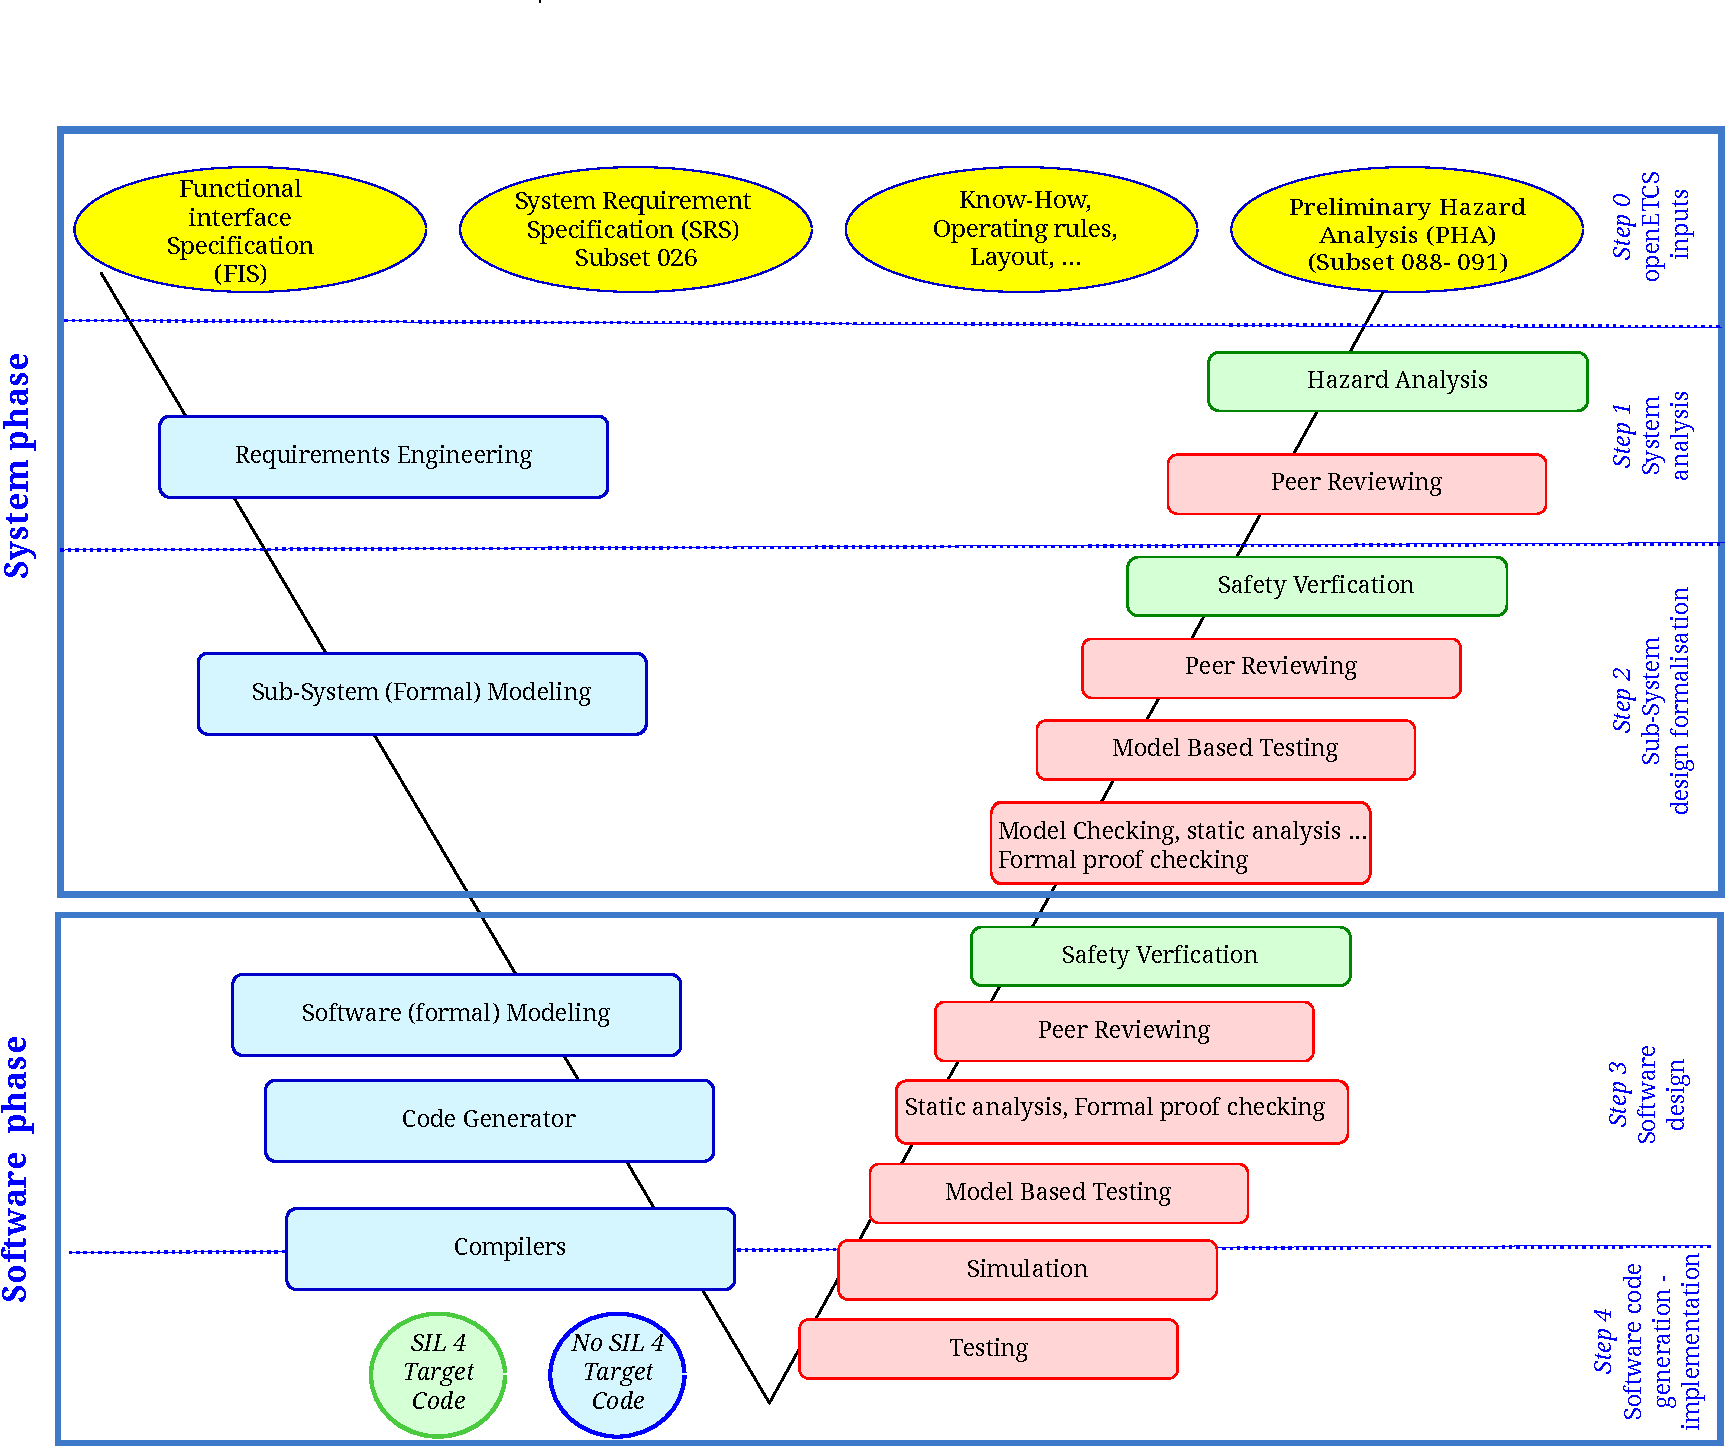
\includegraphics[width=\textwidth]{images/WholeProcess_Activities}
  \caption{openETCS Process Tool chain activities}
  \label{fig:openETCSActivities}
\end{figure}

\todo[inline]{add description of each activities}

%----------------------------------------------------
\section{Management tools}
%----------------------------------------------------
\todo[inline] {add the list of the management tools and a description}
\begin{itemize}
\item Version Management\\
Version management of the artifacts and the openETCS glue code 
\item Tool version Management \\
Keep track of the compatible and status version of each tools. 
\item Collaborative work
\item Project  Management
\item Build system
\item Non regression test
\item Configuration Manger to manage modification and change in tools
\end{itemize}



%%% Local Variables: 
%%% mode: latex
%%% TeX-master: "WP7-Toolchain_architecture"
%%% End: 


%----------------------

\section{OpenETCS Tool chain Life Cycle}
\label{sec:lifecycle}
This part defines the development of the tool chain itself. It defines
the steps to achieve for the implementation of the tool chain.

%----------------------
\subsection{OpenETCS Tool chain use of \gls{COTS}}
To design the life cycle defined in the previous section, the tool chain will
use the components selected by the WP7.  The tool chain will intensively use 
\gls{COTS} application to reduce   the cost for the development of the
\gls{OBU}.

The decision on the selection of means of description, tools and tool platform
are defined in the document \cite{D7.1}. The selection of the secondary tools,
e.g. the choice of verification and validation tools are described in \cite{}.

\subsection{OpenETCS Tool chain development}
The tool chain development will follow the SCRUM process.
The following activities will be covered  by the tool chain development.
\begin{itemize}
\item openETCS tool chain architecture specification\\
Definition of the tool chain composition 
\item openETCS tool chain design specification \\
Definition of how the tool chain is implemented including the
definition of the interoperability mechanism
\item Software development\\
Implementation of the tool chain in particular for the need of tool interoperability
\item Test and verification plan\\
Definition of how to test the tool chain.
\end{itemize}

The tool chain specification is out of the scope of the document. It
has been defined by the WP2, the requirements are listed in Appendix \ref{app:wp2req}.
%%% Local Variables: 
%%% mode: latex
%%% TeX-master: "dev_process"
%%% End: 

%----------------------

\section{OpenETCS Tool chain Development Environment}
\label{sec:env}
The tool chain development will follow the Quality assurance plan \cite{D1.3.1}.
\subsection{Development environment}
Any GNU (or windows) system running on a PC may be used. \gls{IDE}  such as Eclipse may
also be used. 
The tool chain should be under the GIT  version control system
\cite{Chacon:2009}.


To allow robust distributed development, the  environment provides~:
\begin{itemize}
\item  a continuous automated build system,
\item an issue tracker,
\item a request/extension tracker,
\item a backlog
\item a  documentation system.

\end{itemize}
The environment will also provides the infrastructure for a SCRUM development.
The version management within the tool chain 

\subsection{Design Method}
The tool chain will be designed with SysML (\cite{SysML}) Block
diagram with associated interface specifications following the SysML syntax.
The interface will provide the set of artifacts produced or consumed by each tools.

More information may be added to the tool chain model in
order to facilitate the design, the certification and the analysis  of
the openETCS tool chain following the approach
\cite{slotosch_model-based_2012} or \cite{asplund_towards_2012}.

\subsection{Tool chain Development}
Following the scrum process, there will be regular releases for the tool chain.

The tool chain is the integration of  tools, thus the tool chain development
takes care of all the aspects of the tool integration problem (see  
\cite{wasserman_tool_1990}): (1) Platform integration, (2) Data integration,
(3) Presentation integration, (4) Control integration, and (5) Process
integration.
The point (1) is resolved by the choice of the tool platform. The point (5) is
addressed during the design phase of the tool chain.

It has been design that the tool platform hosting the tools will be
Eclipse with Eclipse modeling framework (\gls{EMF}) plug-in. 
To ensure a good  integration, the tool chain development should follow these steps:
\begin{enumerate}
\item Register tool in Eclipse (3)
\item Defining the communication with other tools: method of data exchange (2),
  Control Integration (4)
\end{enumerate}


Furthermore, each tool should register to the tool version
manager. The tool version manager is responsible to keep track of the
version and/or changes of tools and provides the list of compatible
tools versions. 



\subsection{Tool chain  verification}
The validation and verification plan of the tool chain is described in the
a separate  document \cite{}.



\begin{btSect}{biblio}
\section{References}
\btPrintAll
\end{btSect}


\appendix

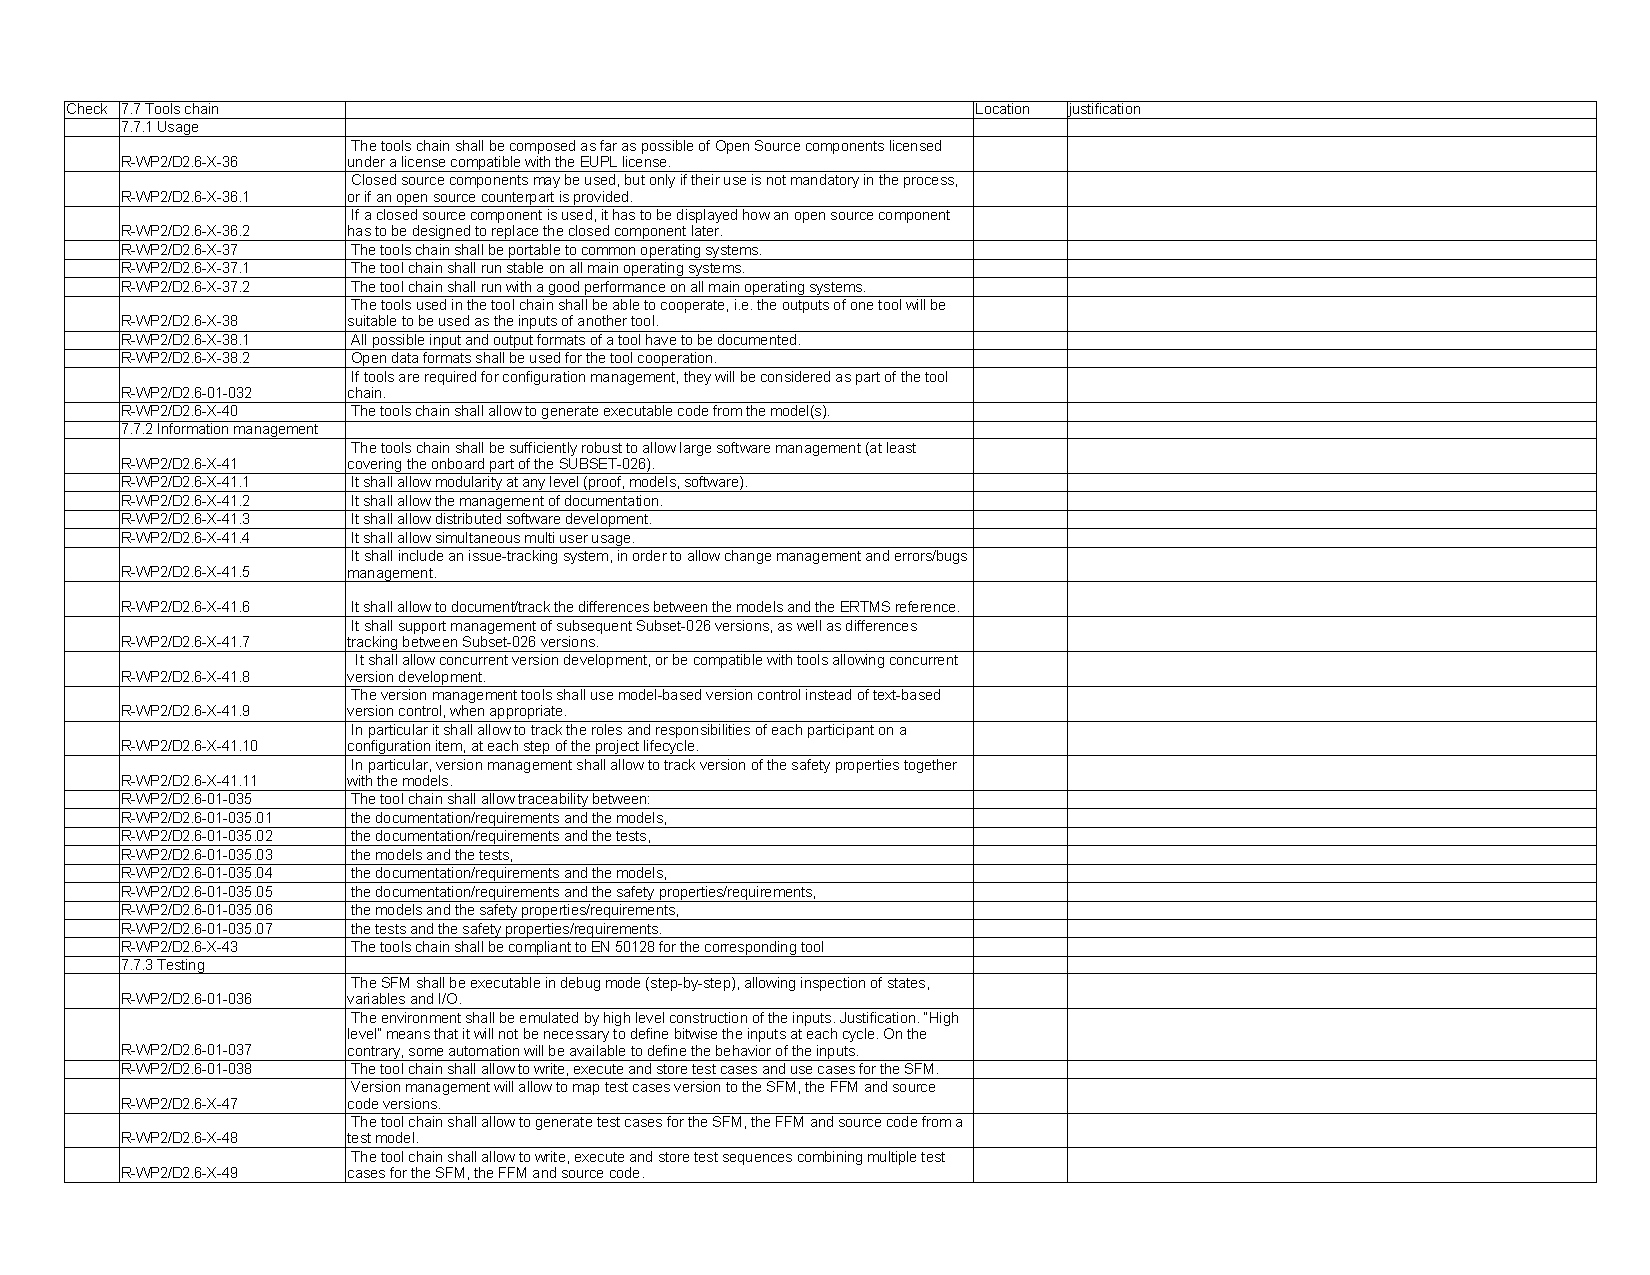
\includepdf[pages={1},landscape=true,pagecommand=\section{WP2 requirements}\label{app:wp2req}]{req_D2_6.pdf}

\includepdf[pages={2},landscape=true,pagecommand={}]{req_D2_6.pdf}


%===================================================
%Do NOT change anything below this line

\end{document}

% LocalWords:  metadata
